\section{Engagement de la cible lors du CAS} % 2. Close Air Support Target Engagement

Cette section décrit les procédures standard lors du \gls{cas}. Bien que certaines opérations nécessitent des procédures spécifiques, le personnel impliqué dans le \gls{cas} doit être familier avec le format standard.

\subsection{Création du briefing par le J-TAC} % a. JTAC Actions for Developing a CAS Brief.
Une fois la cible désignée par le \gls{gc}, le \gls{jtac} doit effectuer les actions décrites ci-dessous.

Le processus commence à la fin et progresse à reculons, en commençant par la cible, de manière à permettre au \gls{jtac} d'établir un \gls{gp}, un \gls{cb}, ainsi que les remarques/restrictions dans un ordre logique.

Cependant, chaque étape a une influence sur les autres, et il se peut qu'il faille revenir sur un point déjà établi durant le processus. Par exemple, le \gls{sead} peut avoir une influence sur le \gls{gp}.


\subsubsection{Rassembler les informations à propos de la cible.}%(1) Develop Targeting Data

Il y a quatre informations dont le \gls{jtac} a absolument besoin pour planifier son attaque: l'élévation de la cible, sa description, sa position, et la position des unités alliées.


\begin{e1}
	
	\itemt{Élévation de la cible (ligne 4).}{
		Par défaut, l'élévation est exprimée en pieds au dessus de la mer (ft \gls{msl}).
		
		Si le \gls{jtac} choisit d'utiliser une autre unité de mesure, cela devra être clairement signifié.
	}

	\itemt{Description de la cible (ligne 5).}{
		La description de la cible doit être concise et précise (par ex. ``5 chars dans un champ'').
		
		Le \gls{jtac}/\gls{faca} doit éviter d'utiliser des descriptions compliquées ou des termes qui risquent de ne pas être compris par les pilotes.
		
		Cependant, la description doit rester spécifique. si le \gls{gc} veut attaquer une \gls{hvt} qui se trouve dans un building à deux étages, il devra spécifier "\gls{hvt} dans building à 2 étages", et pas seulement "building à 2 étages".
	}
	
	\itemt{Position de la cible (ligne 6).}{
		Le \gls{jtac}/\gls{faca} doit évaluer la précision minimale nécessaire pour les coordonnées de la cible pour accomplir les objectifs du \gls{gc}. Il ne faut pas perdre trop de temps à raffiner les coordonnées de la cible et prendre le risque de retarder l'action des appareils de \gls{cas} si l'approximation actuelle de la position suffit à exécuter la mission.
		
		Par exemple, un largage de bombe guidée laser depuis un émetteur au sol demandera des coordonnées beaucoup moins précises qu'une largage de \gls{jdam}.
		
		Il existe plusieurs méthodes pour déterminer la position de la cible:
	}
	
	\begin{e2}
		
		\itemt{Association du terrain et d'une carte.}{
			Le moins précis, mais rapide et efficace en fonction de la situation.
		}
		
		\itemt{\gls{lrf} couplé au \gls{gps} et/ou la boussole.}{
			Sujet à l'imprécision de la boussole, et au brouillage \gls{gps}. Si le brouillage \gls{gps} est possible, une autre méthode devra être utilisée.
		}
		
		\itemt{Logiciel de ciblage}{La méthode la plus précise.}
		
		\itemt{Coordonnées dérivées des images de reconnaissance.}{}
		
	\end{e2}
	
	\itemt{Positions alliées (ligne 8).}{
		La positions des unités alliées au sol sont données à partir de la position de la cible. La direction est donnée de manière cardinale ou sous-cardinale (N, NE, E, SE, S, SW, W, NW), et la distance est exprimée en mètres.
		
		L'observateur ou le \gls{jtac} peuvent ne pas être l'unité alliée la plus proche de la cible.
	}
	
	\itemt{Effet souhaité par le \gls{gc}.}{
		L'effet souhaité par le \gls{gc} est déterminé en parlant avec lui.
		
		Le \gls{jtac} doit offrir au \gls{gc} une estimation réaliste des possibilités en fonction des appareils disponibles, de l'armement embarqué, et de son expertise.
	}
	
\end{e1}

\subsubsection{Requête de CAS} %(2) Request Air Support

\begin{e1}
	\item Une fois que la position de la cible a été grossièrement estimée, le \gls{jtac} doit envoyer la demande de \gls{cas} le plus vite possible, pour prendre en compte le temps nécessaire avant l'arrivée des appareils. Il ne faut pas retarder l'envoi de la demande pour augmenter la précision des coordonnées de la cible.
	
	\important{Il ne faut jamais utiliser les coordonnées des unités alliées comme coordonnées cible dans une demande de \gls{cas}.}
\end{e1}

\subsubsection{Création du game plan} %(3) Develop Game Plan 221

Au minimum, le \gls{gp} contiendra le type de contrôle et la méthode d'attaque.

D'autres informations peuvent être intégrée au \gls{gp} ou être ajouté plus tard aux remarques du \gls{cb}: les intentions du \gls{gc}, l'effet désiré, ou l'intervalle entre les appareils dans le cas d'une attaque simultanée par plusieurs éléments \gls{cas}.

Dans le cas d'attaques séquentielles (\gls{sead}, marquage), une attention particulière devra être apportée à l'établissement de la séparation entre les appareils.

L'objectif du \gls{jtac} n'est pas de dicter aux appareils de \gls{cas} les tactiques à employer, mais de fournir un plan qui correspond aux intentions du \gls{gc}.

\begin{e1}
	
	\itemt{Déterminer l'effet désiré.}{
		La première étape consiste à déterminer l'effet désiré et la manière de créer cet effet.
		
		Les facteurs à prendre en compte sont:
	}
	
	\remark{
		\begin{e2}[2em]
			\item Composition de la cible (blindage).
			\item Répartition de la cible (centré sur un point ou dispersé).
			\item Position (dégagée ou protégée).
			\item Dégâts collatéraux potentiels.
			\item Proximité des unités alliées.
		\end{e2}
	}
	
	Il faudra aussi prendre en compte le type d'appareil \gls{cas}, leur emport probable, leurs systèmes de visée et de guidage, la façon dont l'armement peut être tiré, la menace dans et aux alentours de la zone,  et le temps nécessaire au déploiement de l'armement.
	
	Le \ja{} doit avoir une connaissance minimale de l'effet des armements, et estimer les risques. Si ces risques sont élevés, une coordination avec le \gls{gc} peut s'avérer nécessaire.
	
	Les pilotes peuvent conseiller le \ja{} dans son choix de l'armement et de la méthode de tir.
	
	\itemt{Choisir le type de \gls{tac}.}{
		Le type de \gls{tac} dépend de l'armement employé, de la meilleur manière de réduire les risques, de la vitesse de l'engagement et de la capacité du \gls{jtac} à voir la cible et/ou l'appareil qui attaque.
	}
	
	\itemt{Choisir la méthode d'attaque (\gls{boc} ou \gls{bot}).}{
		La méthode d'attaque est choisie de manière à permettre l'attaque la plus rapide possible, en fonction du type de cible, de la façon dont sera acquise la cible, et de la situation.
	}
	
	\itemt{Planifier l'intervalle entre les appareils.}{
		Le \gls{jtac} peut demander un intervalle spécifique entre les attaques, en fonction de la cible, des menaces, des activités alliées, de la déconfliction artillerie/\gls{sead}/laser, de l'armement utilisé, des restrictions, de la météo, etc.
		
		Les pilotes se doivent d'adapter leur tactiques pour respecter le timing et les intervalles imposés.
	}
	
	\begin{e2}
		
		\itemt{Attaque simultanée.}{
			Tous les appareils délivreront leur armement de manière à créer un effet simultané.
			
			Cette méthode minimise l'exposition des appareils aux menaces et offre à l'ennemi un temps de réaction très court.
			
			C'est la méthode optimale pour engager des cibles multiples, tout particulièrement des unités mobiles qui pourraient fuir après la première attaque.
			
			Le principal désavantage de cette méthode est l'impossibilité de corriger ou d'annuler le tir entre les impacts et la diminution du support mutuel entre les appareils qui attaquent.
			
			\important{Un attaque simultanée nécessite que les appareils utilisent des codes laser différents.}
		}
		
		\itemt{Attaque séquentielle.}{
			Les appareils attaquent un à la fois, avec un intervalle spécifique entre les attaques, basé sur le temps nécessaire à l'acquisition de l'appareil précédent, la durée de vol de l'arme employée, le temps nécessaire au dégagement visuel de la zone attaquée (fumée, fragments, etc.), et le temps nécessaire à évaluer l'efficacité de la frappe précédente et le besoin d'une nouvelle frappe.
			
			Quelques guides pour les attaques séquentielles:
		}
		\begin{e3}
			\item 30 secondes pour un contrôle de \gls{typeone} avec des bombes lisses.
			\item 1 minute pour des \gls{lgb} délivrées à altitude moyenne.
			\item Plus de deux minutes pour décider de la ré-attaque lors de l'emploi de \gls{pgm} à haute ou moyenne altitude.
		\end{e3}
		
		\itemt{Développer un plan d'utilisation des senseurs.}{
			Le \ja{} doit prendre en compte le temps nécessaire à la mise en oeuvre et à l'utilisation des différents senseurs embarqués.
			
			\todo[inline]{Lien vers la section ISR du chapitre 3 (vide ATM)}
		}
	\end{e2}
\end{e1}

\subsubsection{Détermination du type de marque et de l'aide à la corrélation} %(4) Determine/Coordinate Mark/Aid to Correlation 222

\begin{e1}
	
	\itemt{\glsfull{boc}.}{}
	
	\begin{e2}
		\item Pas de marque nécessaire (ligne 7: "No mark").
		
		\item Si le \gls{tac} est utilisé avec des \gls{lgw}, le call-sign de l'unité qui fournit le \gls{tac} et le code laser seront fournis.
		
		Exemple de ligne 7: "Blackjack laser, code 1688".
	\end{e2}
	
	\itemt{\gls{bot}.}{
		La marque dépendra de l'appareil qui attaque.
	}
	
	\itemt{\gls{bot} et contribution d'une tierce partie.}{}
	
	\begin{e2}
		
		\itemt{Tierce partie.}{
			Suite l'expansion des technologies déployées sur le champ de bataille, le \gls{jtac} peut décider de recourir à une tierce partie (unité \gls{recce}, sniper, appareils équipés d'un émetteur laser, etc.) pour aider à l'obtention des coordonnées ou de la position de la cible, à l'attaque terminale ou à l'établissement du \gls{bda}.
			
			De ce fait, la corrélation entre les pilotes ou le \ja{} et ces parties tierces sera également nécessaire.
		}
		
		\item{Considérations.}{}
		
		\begin{e3}
			\item Les pilotes utilisent généralement une combinaison de senseurs et leurs yeux pour acquérir les marques et les cibles.
			
			Par exemple, un pilote de \gls{fw} peut utiliser un \gls{lst} pour traquer l'origine du ciblage laser du \gls{jtac} et ainsi obtenir sa position.
			
			Les \glspl{jtac} doivent être familiers avec les capacités des senseurs et utiliser des marques qui utilisent ces capacités.
			
			\item Le \gls{jtac} doit toujours avoir en réserve un plan de marquage alternatif.
		\end{e3}
		
		\itemt{Types de marque et \gls{tgo}.}{}
		
		\begin{e3}
			
			\itemt{Marquage laser.}{
				La marque laser utilise un \gls{ltd} pour fournir l'énergie laser au \gls{lst} de l'appareil.
				
				Le \gls{ltd} peut se trouver au sol ou embarqué dans un autre appareil.
			}
			
			\begin{e4}
				\item Avantages:
				\begin{e5}
					\item Excellente corrélation de la position de la cible si la géométrie correcte est utilisée.
					\item Peut être utilisé de jour comme de nuit.
				\end{e5}
				\item Désavantages:
				\begin{e5}
						\item Nécessite un \gls{ltd} et un \gls{lst}.
						\item Demande de la coordination géométrique pour le \gls{lst} ne traque pas le \gls{ltd} (l'origine du pointage).
						\item Le marquage laser depuis le sol est souvent difficile, particulièrement lorsque l'unité qui effectue le pointage est sous le feu ennemi.
						\item Un premier passage d'acquisition de la marque est parfois nécessaire.
				\end{e5}
				\important{Lors du marquage laser depuis le sol, un \gls{fah} sera obligatoirement donné, de manière à renforcer l'établissement de la géométrie correcte.}
			\end{e4}
			
			\itemt{Marquage infrarouge (\acrshort{sparkle}).}{
				Les pilotes utiliseront leur \gls{nvg} pour acquérir la cible.
			}

			\makebox[\textwidth]{\centering 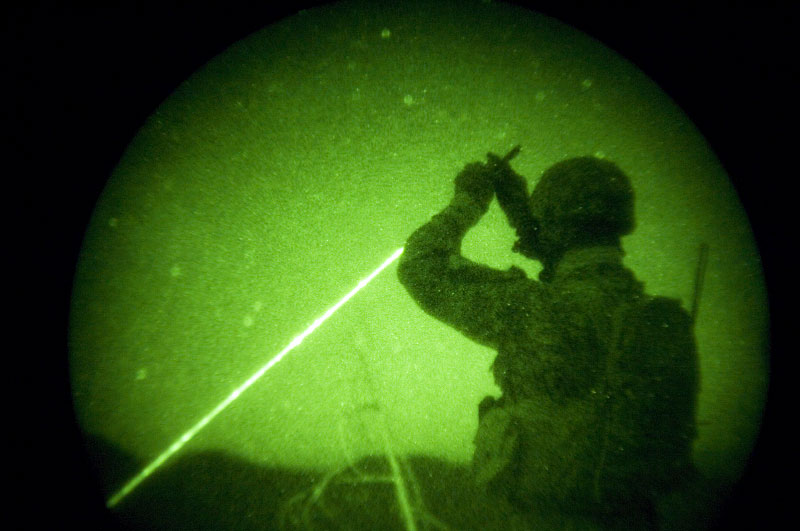
\includegraphics[width=0.5\textwidth]{niceties/ir}}

			\important{Les pilotes doivent appeler "VISUEL SPARKLE", "TALLY SPARKLE" ou "CONTACT SPARKLE" quand un marquage infrarouge est utilisé à partir du sol.}
			\begin{e4}
				\item Avantages:
				\begin{e5}
					\item Rapide.
					\item Le \gls{jtac} a la confirmation visuelle que le pilote a bien acquis la cible correcte.
				\end{e5}
				\item Désavantages:
				\begin{e5}
					\item De nuit seulement.
					\item Requiert de la coordination géométrique pour s'assurer que le pilote a bien acquis la fin du faisceau infrarouge et non pas sa source.
					\item S'il y a plusieurs pointeurs \gls{ir} près d'une même cible, il devient difficile pour le \gls{jtac} de déterminer si le pointeur se trouve bien sur la cible à cause du phénomène de ``diffusion'' dans les \gls{nvg}.
					\item Si l'ennemi dispose également de \gls{nvg}, l'utilisation d'\gls{ir} expose l'opérateur et supprime le facteur de surprise.
				\end{e5}
			\end{e4}
			
			\itemt{Walk-on infrarouge (\acrshort{sparkle}).}{
				Diriger, par une discussion entre le \gls{jtac} et le pilote, le pointeur infrarouge de l'appareil sur la cible.
			}
			
			\begin{e4}
				\item Avantages:
				\begin{e5}
					\item Ne nécessite pas que l'opérateur au sol révèle sa position aux unités ennemies équipées \gls{ir}.
					\item Le \gls{jtac} a la confirmation visuelle que le pilote a bien acquis la cible correcte.
				\end{e5}
				\item Désavantages:
				\begin{e5}
					\item De nuit seulement.
					\item Les ennemis équipés de \gls{nvg} sauront qu'ils sont pris pour cible.
					\item Du fait de la différence de perspective, il peut être très difficile de diriger efficacement le pointeur \gls{ir}.
				\end{e5}
			\end{e4}
			
			\itemt{Marquage à partir d'un \gls{trp}.}{}
			
			\begin{e4}
				\item Avantages:
				\begin{e5}
					\item Prêt rapidement si le pilote connaît le \gls{trp}.
					\item De jour comme de nuit.
					\item Offre un point de référence commun pour le talk-on.
				\end{e5}
				\item Désavantages:
				\begin{e5}
					\item Nécessite le pilote connaisse le \gls{trp}.
				\end{e5}
			\end{e4}
			
			\itemt{Marquage \gls{idf} (fumigène).}{}
			
			\begin{e4}
				\item Avantages:
				\begin{e5}
					\item De jour comme de nuit (obus phosphorescents ou lumineux).
					\item Le \gls{jtac} ne doit pas dévoiler sa position.
					\item Offre un point de référence commun pour le talk-on.
				\end{e5}
				\item Désavantages:
				\begin{e5}
					\item Prend du temps à coordonner.
					\item Le manque de précision implique souvent une correction supplémentaire à partir de la marque.
					\item Le tire indirect implique une déconfliction supplémentaire.
					\item Le \gls{fov} des senseurs peut être un problème si la marque se trouve en dehors.
					\item L'illumination de nuit sature les \gls{nvg}.
					\item Sacrifie l'effet de surprise.
				\end{e5}
			\end{e4}
			
			\itemt{Marquage par feu direct.}{
				Le marquage par feu direct utilise un tir direct (munitions traçantes ou grandes fumigènes) pour diriger l'attention du pilote sur les impacts et révéler ainsi la cible.
			}
			
			\begin{e4}
				\item Avantages:
				\begin{e5}
					\item Facilement accessible:
				\end{e5}
				\item Désavantages:
				\begin{e5}
					\item Risque de dommages collatéraux.
					\item Difficulté pour les \gls{rw} d'acquérir visuellement la marque de jour.
					\item Difficulté pour les \gls{fw} d'acquérir visuellement la marque de jour comme de nuit.
					\item Le \gls{fov} des senseurs peut être un problème si la marque se trouve en dehors.
					\item L'illumination de nuit sature les \glspl{nvg}.
					\item Sacrifie l'effet de surprise.
				\end{e5}
			\end{e4}
			
			\itemt{Considérations pour le marquage de nuit:}{}
			\begin{e4}
				\item La visibilité limitée et le manque de perspective rend la corrélation de nuit difficile.
				\item L'illumination du champ de bataille doit être planifiée de manière à ne pas saturer les \glspl{nvg}.
			\end{e4}
			
			\itemt{Marques d'opportunité.}{
			N'importe quoi sur le champ de bataille peut servir de marque; un bâtiment en feu, le trafic routier, etc.
			}
			
		\end{e3}
	\end{e2}
\end{e1}
	
\subsubsection{Détermination la géométrie d'attaque} %(5) Develop Attack Geometry 227

Les \glspl{jtac} doivent prendre de nombreux facteurs en compte lors de l'établissement de la géométrie d'attaque:

\begin{e1}
	\itemt{\glsfull{fah}}{
		Voir Chapitre 3, \smallref{tofah} pour plus d'informations sur le \gls{fah}.
	}
	
	\begin{e2}
		\item Le \ja{} doit éviter d'établir un \gls{fah} qui fait passer l'appareil en attaque au-dessus d'une position occupée par un allié (sol,\gls{bp}, \gls{ha}, \ldots{}).
		
		\item Le \ja{} doit prendre en compte le fait que certains appareils ont la capacité de tirer à gauche ou à droite de leur axe longitudinal (canon mobile, armes intelligentes, \ldots{}).
		
		\item le \ja{} doit prendre en compte la possibilité de ricochets ou de rebonds, et planifier le \gls{fah} parallèle à la \Gls{flot} si possible.
		
	\end{e2}
	
	\item La déconfliction latérale ou verticale avec les autres appuis-feu peut s'avérer nécessaire si la déconfliction horaire n'a pas été possible.
	
	\item Géométrie laser.
	
	\item Orientation/disposition de la cible:
	
	\begin{e2}
		
		\item Pour les cible alignées, le \gls{fah} doit de préférence être aligné avec les cibles.
		
		\item Pour les cibles en mouvement, le \gls{fah} doit de préférence être aligné sur l'axe de progression de la cible.
		
		\item Obstacles:
		
		\begin{e3}
			
			\item Canyons urbains: le \gls{fah} doit de préférence être aligné sur les canyons urbains.
			
			\item Terrain: certains éléments du terrain (montagnes par exemple) peuvent grandement influencer le choix du \gls{fah}.
			
		\end{e3}
		
		\item Météo:
		
		\begin{e3}
			
			\item Vent: un vent de travers de plus de 30kts peut affecter la précision des armes guidées.
			
			Les priorités pour le \gls{fah} sont vent arrière, vent debout, et finalement vent de travers.
			
			\item Position/angle du soleil ou de la lune:
			
			\begin{e4}
				
				\item Il faut éviter de faire attaquer les appareils avec le soleil ou la lune de face.
				
				\item Attaquer le soleil dans le dos fournit une protection supplémentaire contre les \glspl{manpad}.
				
			\end{e4}
			
			\item Nuages:
			
			\begin{e4}
				
				\item Peuvent empêcher le \gls{jtac} de voir les appareils qui attaquent.
				
				\item Peuvent empêcher les appareils qui attaquent de trouver la cible.
				
			\end{e4}
			
		\end{e3}
		
		\item Autres restrictions \glspl{acm}/\glspl{fscm} pré-planifiées.
		
		\item Le \ja{} doit déterminer l'\gls{ip}/\gls{bp} et le plan d'egress de manière cohérente avec la géométrie d'attaque (lignes 1, 2, 3, 9).
		
		Le \ja{} fait son possible pour utiliser des points d'ingress/egress qui n'imposent pas aux appareils de larges virages pour respecter le \gls{fah}.
		
	\end{e2}
	
\end{e1}

\subsubsection{Plan SEAD}%(6) Determine SEAD Requirements/SEAD Plan 229

\begin{e1}
	
	\item S'il n'est pas possible d'éviter la menaces sol-air, un plan \gls{sead} devra être établi.
	
	\item Le \gls{sead} et le \gls{cas} peuvent se retrouver à engager le même groupe cible; il faut alors faire attention à ce qu'il ne s'empêche pas l'un l'autre de travailler.
	
	\item La menace peut également être réduite au moyen de:
	
	\begin{e2}
		
		\item Séparation latéral: employer des armes à longue portée.
		
		\item Séparation verticale: rester au dessus de l'enveloppe de tir de la menace.
		
		\item Masquage terrain:
		
		\begin{e3}
			
			\item Tir pop-up.
			
			\todo[inline]{For examples of SEAD integration, see Appendix E, “Examples of Close Air Support Missions,” Examples 1 and 7.}
			
		\end{e3}
		
	\end{e2}
	
\end{e1}

\subsection{Template d'exécution du CAS}%b. CAS Execution Template. 231

Par sa nature même, l'exécution du \gls{cas} diffère lors de chaque mission.

Les grandes lignes restent cependant toujours les mêmes.

La template suivante fournit un cadre de travail pour le \ja{} et les pilotes.

\remark{Le déroulement présenté ici commence après le décollage, et se termine lorsque la patrouille de \acrshort{cas} est sur le retour.}

\subsubsection{Routing}%(1) Routing/Safety of Flight. 231

Directement après le check-in, le \ja{} doit fournir au pilote une liste des autres \glspl{aos}, leur call-sign, l'altitude à laquelle ils opèrent, et leur fréquence de travail, ce dès que possible.

Le \ja{} doit communiquer au pilote l'espace aérien disponible et la position de l'\gls{ip}/\gls{ha} pour l'attaque.

Lors du check-in initial, le \ja{} donnera, dans l'ordre:

\begin{e1}
	
	\begin{minipage}{\linewidth}
		\itemt{Instructions de transit/Instructions d'attente}{
			Lors du contact initial, le contrôleur donnera au moins une instruction du type ``Maintenez'', de manière à établir le contrôle:
		}
		
		\begin{lstlisting}[caption=Routing: maintenez, label=routingmaintain]
	REDWOLF, maintenez Chevy 14.
		\end{lstlisting}
	\end{minipage}
	
	\begin{e2}
		
		\begin{minipage}{\linewidth}
			\item S'il n'est pas certain de l'altitude actuelle de l'appareil, le \ja{} devra la demander:
			
			\begin{lstlisting}[caption=Routing: demande de position, label=routingask1]
			REDWOLF, donnez position et altitude.
			\end{lstlisting}
		\end{minipage}
		
		\begin{minipage}{\linewidth}
			\item Si un \gls{kh} non-briefé est utilisé, le \ja{} doit donner le point Echo au pilote avant de donner les informations de transit:
			
			\begin{lstlisting}[caption=Routing: keyhole, label=routinkh]
	REDWOLF, Keyhole effectif, point Echo 43 52.1N 042 43.8E, allez Alpha 10km, 500m, rappelez "é"tabli.
			\end{lstlisting}
		\end{minipage}
		
		
	\end{e2}
	
	\begin{minipage}{\linewidth}
		\item S'il n'y a pas d'autre \gls{aos}, cela devra être dit:
		
		\begin{lstlisting}[caption=Routing: pas d'autre AOS, label=routingnoaos]
	REDWOLF, allez sur Chevy, maintenez 500m, vous "ê"tes seul en station.
		\end{lstlisting}
	\end{minipage}
	
	\item Autres informations pour la sécurité du vol:
	
	\begin{e2}
		
		
		
		\begin{minipage}{\linewidth}
			\item Menaces immédiates:
			
			\begin{lstlisting}[caption=Routing: menace immédiate, label=routingthreat]
	REDWOLF, allez de Emily "à" Adder restez en dessous de 100m, ZSU23 "à" proximit"é"de l'usine 34, vous "ê"tes seul en station.
			\end{lstlisting}
		\end{minipage}
		
		\item Fait marquant à propos de la météo ou du terrain.
		
	\end{e2}
	
	\item Pour maintenir sa \gls{sa} quant à la position des différents appareils, le \ja{} pourra demander des mises à jours de statut durant la phase de routing.
	
	\begin{minipage}{\linewidth}
		\item Exemples d'appels de routing et sécurité:
		
		\begin{lstlisting}[caption=Routing: exemple 1, label=routingex1]
	REDWOLF, allez sur Frog, maintenez 300m, sur Frog descendez et maintenez 100m, rappelez "é"tabli, standby pour le check-in, vous "ê"tes seul en station.
		\end{lstlisting}
		
		\begin{lstlisting}[caption=Routing: exemple 2, label=routingex2]
	REDWOLF, allez sur la HA Betty, restez en dessous de 1000m, artillerie alli"é"e 12 tire, direction 340, vous "ê"tes seul en station.
		\end{lstlisting}
	\end{minipage}

\end{e1}

\subsubsection{Check-in}%(2) CAS Aircraft Check-In.  232

La procédure de check-in est essentielle pour le passage des informations entre les pilotes et les agences de contrôle.

Les agences de contrôle doivent tenir les pilotes à jour des évolutions de la situation durant le transit vers la zone de combat.

C'est pourquoi il est important que le \ja{} tiennent les agences de contrôle informées de la situation, de façon à ce que les appareils arrivent sur zone disposent déjà des dernières informations.

\begin{e1}
	
	\begin{minipage}{\linewidth}
		\item Le \ja{} choisit le moment auquel les appareils \gls{cas} envoient leur check-in:
		
		\begin{lstlisting}[caption=Check-in: envoi, label=checkinsend]
	REDWOLF, envoyez votre check-in.
		\end{lstlisting}
	\end{minipage}
	
	\item Il peut y avoir plusieurs raisons pour retarder ou abréger un check-in.
	
	Le \ja{} peut ne pas être prêt, ou en attente de contact par un autre appareil.
	
	Si l'appareil est prévu dans l'\gls{ato}, et que le \ja{} a une copie de cet \gls{ato}, le check-in peut se résumer à ``As fragged'' (comme prévu) ou ``As fragged, with exception: \ldots{}'' (comme prévu, à l'exception de: \ldots{}), pour gagner du temps sur la suite des transmissions.
	
	Si l'appareil doit passer par plusieurs contrôleurs, il peut être judicieux de réserver le check-in complet au \ja{} avec lequel l'attaque finale sera effectuée.
	
	\begin{minipage}{\linewidth}
	\begin{lstlisting}[caption=Check-in: standby, label=checkinstandby]
	REDWOLF, standby check-in, attaque en cours.
	\end{lstlisting}
	\end{minipage}
	
	\begin{minipage}{\linewidth}
	\begin{lstlisting}[caption=Check-in: autre contrôleur, label=checkinothercontrol]
	REDWOLF, PIRATE prendra votre check-in, contactez le sur Isabelle.
	\end{lstlisting}
	\end{minipage}
	
	\item Authentification: si les communications ne sont pas sécurisées, une authentification devra être effectuée. Cfr. \cruderef{dryad}.
	
	\item En fonction de la situation, le \ja{} peut demander à n'avoir que certaines parties du check-in.
	
	\begin{minipage}{\linewidth}
		\item Format du check-in:
		\begin{figure}[H]
			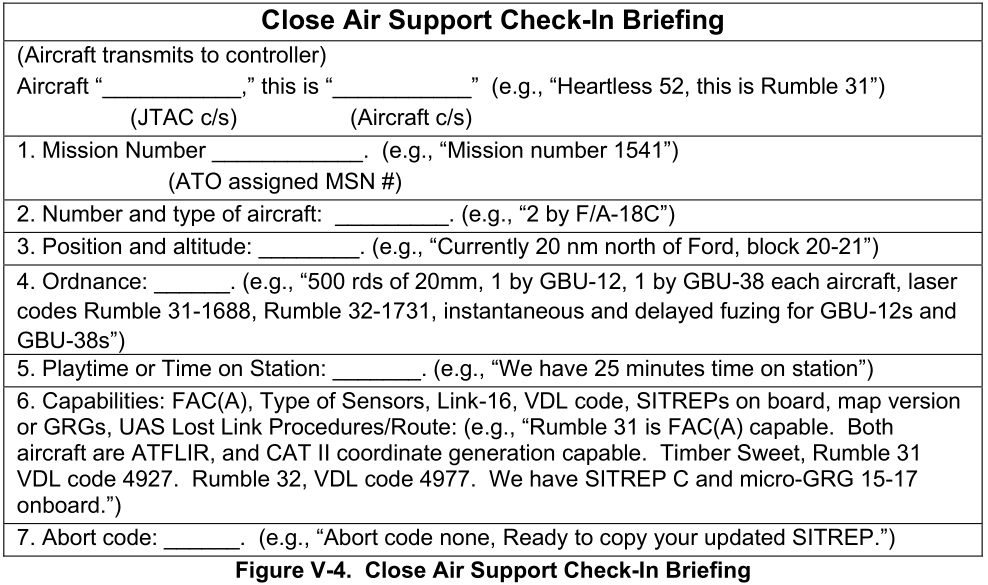
\includegraphics[width=\textwidth]{checkin.png}
			\caption{Format check-in.}
			\label{fig:checkin}
		\end{figure}	
	\end{minipage}
	
	\begin{minipage}{\linewidth}
		\itemt{Format du check-in:}{}
		\begin{lstlisting}[caption=Check-in: partiel, label=checkinpart]
	REDWOLF, pas de check-in complet, donnez armement et play-time.
		\end{lstlisting}
	\end{minipage}
	
	\begin{e2}
		\item Numéro de mission.
		\item Nombre et type d'appareils.
		\item Position et altitude.
		\item Armement:
		\begin{e3}
			\item Code laser pour les \glspl{lgb}.
			\item Type.
			\item Configuration de mise à feu (instantanée, retardée, au dessus du sol).
		\end{e3}
		\item Play-time/\gls{tos}.
		\item Capacités:
		\begin{e3}
			\item Dernier SITREP/AO Update reçu.
			\item Version du \gls{grg} à bord
			\item Capacités \gls{faca}.
			\item Capacité des senseurs.
		\end{e3}
		\item Code Abort:
		\begin{e3}
			\item Sur un réseau sécurisé, un code Abort n'est pas nécessaire, l'appel ``ABORT, ABORT, ABORT'' suffira.
			\item Sur un réseau non-sécurisé, un mot code sera établi selon les \gls{spins}/\glspl{sop} en place (ex: RAMROD, \hyperref[dryad]{DRYAD}).
		\end{e3}
		\item Si le \ja{} n'est pas familier avec le type d'appareil, il devra maintenant poser les questions en clair de manière à éviter de donner plus tard des instructions impossibles à suivre.
	\end{e2}
\end{e1}
	
\subsubsection{Situation Update}\label[subsubsection]{subsubsec_aoupdatee}%(3) Situation Update 234
	
\begin{e1}
	\item La Situation Update est un outil utilisé pour augmenter la \gls{sa} de tous.
	
	La Situation Update peut inclure:
	
	\begin{e2}
		
		\item Activités ennemies.
		\item Activités des menaces.
		\item Situation alliée.
		\item Remarques.
		\item Météo.
		\item Dangers.
		
	\end{e2}
	
	\item Exemples d'AO Update:
	
	\efig{aoupdate1}{AO Update: exemple 1.}
	
	\efig{aoupdate2}{AO Update: exemple 2.}
	
	\begin{e2}
		\item La longueur de l'AO Update doit être adaptée en fonction du temps disponible.
		
		L'objectif de l'AO Update est de donner au pilote une \gls{sa} suffisante pour remplir sa mission.
		
		Les AO Update qui sont lues trop vite, sont trop longues, ou donnent des informations inutiles, font perdre du temps et contribuent à réduire la \gls{sa} de tous.
		
		Une AO Update particulièrement longue doit être fragmentée en plusieurs transmissions.
		
		\item Lorsque c'est possible, l'AO Update doit être transmises aux agences de contrôle, pour qu'elles puissent en informer les appareils en transit.
		
		Aussi, la transmission de l'AO Update peut être déléguée au \gls{faca}/\gls{taca}, pour permettre au \gls{jtac} de se concentrer sur le \gls{tac}.
		
		\itemt{Codage des AO Updates}{
			Les AO Updates reçoivent un codes alphanumérique, qui est transmis en même temps que l'AO Update.
			
			Cela permet au \ja{} de savoir si un pilote dispose de la dernière AO Update.
		}
		
		\begin{minipage}{\linewidth}
			\itemt{Format du check-in:}{}
			\begin{lstlisting}[caption=AO Update: code, label=aoupdatecode]
	REDWOLF ici MAGIC, avec AO Update Charlie, rappellez pr"ê"t "à" copier.
	...
	PIRATE ici REDWOLF, pour le check-in.
	...
	PIRATE ici REDWOLF, ..., AO Update Bravo "à" bord.
			\end{lstlisting}
		\end{minipage}
		
	\end{e2}
	
\end{e1}
	


\subsubsection{Game-plan}%(4) Game Plan.  237

Le Game-plan est une méthode concise d'informer les pilotes des intentions du \ja{}.

\efig{gameplan}{Game-plan: exemple.}

\begin{e1}
	\item S'il reste des questions quant aux capacités de l'appareil, elles doivent être élucidées.
	
	\begin{minipage}{\linewidth}
		\item Le Game-plan est utilisé pour les attaques simples ou multiples.
		
		Si plusieurs appareils sont prévus pour l'attaque, il faut essayer de ne transmettre le Game-plan qu'une seule fois:
		\begin{lstlisting}[caption=Game-plan: transmission unique, label=gameplansingletx]
	REDWOLF et BOURDON, dans l'ordre, rappellez pr"ê"t "à" copier le Game-plan.
		\end{lstlisting}
	\end{minipage}
	
	\item Pour les attaques multiples, le termes ``dans l'ordre'' (in order) est utilisé pour indiquer l'ordre dans lequel les appareils doivent répondre au \ja{}.
	
	Pour les attaques multiples, les éléments suivants doivent être renseignés:
	
	\begin{e2}
		
		\item Type d'attaque coordonnée:
		
		\begin{e3}
			
			\item Type d'attaque: combinée ou par secteurs
			
			\item Timing: simultanée, séquentielle, ou aléatoire.
			
		\end{e3}
		
		\item Conduite de l'attaque:
		
		\begin{e3}
			
			\item Attaque combinée: méthode de séparation (visuelle, temporelle, altitude).
			
			\begin{minipage}{\linewidth}
				
				\item Attaque par secteurs: secteurs respectifs pour chaque élément.
				
				Par exemple:
				
				\begin{lstlisting}[caption=Game-plan: attaque par secteurs, label=gameplansector]
	REDWOLF et BOURDON, ce sera une attaque simultan"é"e par secteur, REDWOLF "à" l'est, BOURDON "à" l'ouest. REDWOLF, rappellez pr"ê"t pour le Game-plan.
				\end{lstlisting}
			\end{minipage}
			
		\end{e3}
		\begin{minipage}{\linewidth}
		\item Le \ja{} donnera au premier élément le Game-plan complet, le CAS-brief, les remarques et les restrictions avant de donner le Game-plan aux second élément.
		
		Le second élément doit écouter cette transmission: si certains éléments sont communs, le \ja{} donnera au second élément les différence uniquement.
		
		Par exemple:
		
		\begin{lstlisting}[caption=Game-plan: game-plan commun, label=gameplancommon]
	REDWOLF et BOURDON, ce sera une attaque s"é"quentielle combin"é"e, REDWOLF attaque en premier, suivi par BOURDON 2 minutes apr"è"s impact. REDWOLF, rappellez pr"ê"t pour le Game-plan.
		\end{lstlisting}
		\end{minipage}
		
		\item Pendant le briefing d'attaques multiples, le \ja{} peut appeler ``standby read-backs'', pour demander au pilote de ne pas effectuer le read-back immédiatement après la transmission des informations.
		
		Le \ja{} demandera un read-back séquentiel de tous les pilotes une fois le briefing terminé.
		
		\item Marque laser par une tierce partie: lorsqu'une tierce partie assure la marque laser, son call-sign et le code laser utilisé sera donné en Ligne 7.
		
		
	\end{e2}
	
\end{e1}

\subsubsection{CAS-brief}\label[subsubsection]{subsubsec_nineline} [%(5) CAS Brief 241

Le \ja{} utilisera un format standard pour transmettre le CAS-brief, d'application pour les \glspl{fw} comme pour les \glspl{rw}.

Ce format est appelé \glsfull{9l}.

La \gls{9l} est transmise d'une traite.

Les en-têtes des lignes ne sont pas transmis.

Le format est le suivant:

\efig{9line}{Format 9-Line}

\remark{L'\citetitle{atp63} stipule qu'un \gls{faca} OTAN passera l'intitulé des lignes, pour chaque ligne.}

\begin{minipage}{\linewidth}
	Si les lignes 1-3 sont abrégée, la \gls{9l} commencera par le mot ``Élévation''.
	\begin{lstlisting}[caption=9-Line: lignes 1-3 abbrégée, label=9labbr]
	Depuis la verticale. Elevation, 324... .
	\end{lstlisting}
\end{minipage}
	


\begin{minipage}{\linewidth}	
	Le \ja{} peut avertir le pilote avant la transmission de la \gls{9l}:	
	\begin{lstlisting}[caption=9-Line: avertissement, label=9loavert]
	REDWOLF, rappellez pr"ê"t "à" copier la 9-Line.
	\end{lstlisting}
\end{minipage}
	
\begin{e1}
	\itemt{Ligne 1: \glsfull{ip} ou \glsfull{bp}}{
		L'\gls{ip} est le point de départ de l'attaque.
		
		Pour les \glspl{rw}, la \gls{bp} est l'endroit où commencent les attaques.
		
		La ligne 1 contient:
	}
	
	\begin{e2}
		
		\item Nom de \gls{ip}/\gls{bp}.
		
		\item Position de la \gls{ip}/\gls{bp} ``jetable'' (par exemple \gls{kh}).
		
	\end{e2}
	
	\itemt{Ligne 2: Cap et offset}{
		Le cap est donné en degrés magnétique de l'\gls{ip} vers la cible, ou depuis le centre de la \gls{bp} vers la cible.
		
		Le \ja{} peut donner un offset s'il le souhaite.
		
		\important{Le cap est donné en 3 chiffres.}
	}
	
	\itemt{Ligne 3 - Distance}{
		Pour les \glspl{fw}, la distance est donnée en miles nautiques, au dixième de mile nautique, entre l'\gls{ip} et la cible.
		
		Pour les \glspl{rw}, la distance est donnée en mètres, entre le centre de la \gls{bp} et la cible.
	}
	
	\itemt{Ligne 4 - Élévation de la cible}{
		L'élévation est données en \gls{ft} \gls{msl}.
	}
	
	\begin{e2}
		
		\item L'élévation est lue comme une séquence de chiffres.
		
		Il est recommandé d'inclure le mot ``pieds'' à la fin pour marquer la transition avec les chiffres de la ligne 5.
		
		\item Les \gls{ft} \gls{msl} sont implicites; si une autre unité ou un autre référentiel sont utilisés, ce devra être spécifié.
		
		\item Si les lignes 1-3 ont été abrégée, la transmission commence par le mot ``Élévation''.
		
	\end{e2}
	
	\itemt{Ligne 5 - Description de la cible}{
		La description de la cible doit être suffisamment spécifique que pour permettre au pilote de l'identifier.
		
		La cible doit être décrite de manière précise et concise en utilisant un langage commun.
		
		Si des précisions sont nécessaire pour identifier une cible spécifique dans un groupe, elles seront données plus tard.
	}
	
	\itemt{Ligne 6 - Position de la cible}{}
	\begin{e2}
		
		\item Le \ja{} peut donner la position de la cible de 3 manières:
		
		\begin{e3}
			
			\item Coordonnées sur la grille.
			
			\item Latitude et longitude.
			
			\item Offset à partir d'un point connu.			
			
		\end{e3}
		
		\item Si la cible est une zone plutôt qu'un point, il faudra donner la position du centre de la zone.
		
		\item Si la cible se compose de plusieurs éléments alignés, le position devra correspondre au point d'impact souhaité.
		
		L'orientation de la la ligne et la distance à couvrir avant et après le point central seront donnée en Ligne 5 ou dans les remarques.
		
		\item Cibles multiples: lors de la transmission de plusieurs Lignes 4 et 6, le \ja{} donnera d'abord un CAS-brief complet, puis ajouter les Lignes 4, 6 et 8 supplémentaires avant les remarques.
		
		\item Si les coordonnées sont passées comme latitude et longitude, les mots ``nord'', ``est'', ``sud'' et ``ouest'' seront lus \textbf{avant} les chiffres.
		
		\item Les points suivants sont à prendre en compte si on utilise une méthode autre que les coordonnées géographiques:
		
		\begin{e3}
			
			\item Pour l'offset à partir du point connu, ce point devra être défini par le contrôleur et acquis par le pilote avant le CAS-brief.
			
			\begin{minipage}{\linewidth}
				
				\item Pour une cible mouvante, il faudra fournir l'axe de progression de la cible, sous forme d'un point d'origine, d'une direction et d'une vitesse.
				
				Le mouvement de la cible devra être évalué en relation avec les unités alliées, et les éléments civils et non-combattants.
				
				En se basant sur ces estimations, les lignes 4, 6 et 8 seront mises à jour avant l'attaque finale.
				\begin{lstlisting}[caption=9-Line: cible mouvante, label=9lmoving]
	REDWOLF, PIRATE, la cible est un v"é"hicule blind"é" isol"é" "à" proximit"é" du pont "à" l'est de la ville, faisant route "à" l'est, environ 30kmh.
				\end{lstlisting}
			\end{minipage}
			
		\end{e3}
		
	\end{e2}
	
	\itemt{Ligne 7 - Marque/Guidage terminal}{
		\begin{e2}
			
			\item Type de la marque: le \ja{} indiquera le type de marque utilisé (par exemple: fumigène, laser, infrarouge).
			
			S'il utilise un laser, le \ja{} en donnera le code.
			
			\item Guidage terminal: lorsqu'une tierce partie assure le guidage terminal de l'arme, le \ja{} donnera son call-sign, le mot ``laser'', et le code laser utilisé.
			
		\end{e2}
	}
	
	\itemt{Ligne 8 - Alliés}{
		Direction cardinale ou sous-cardinale (N, NE, E, SE, S, SW, W, ou NW) et distance en mètre, à partir de la cible, de l'allié le plus proche de la cible.
	}
	
	\itemt{Ligne 9 - Egress}{
		Instructions pour quitter la zone une fois l'attaque terminée.
		
		La direction peut être donnée de manière cardinale à partir d'un point, ou, si la situation le permet, en appelant ``Egress à la discrétion du pilote''.
		
		Le mot ``egress'' sera dit avant de donner les instructions.
		
		L'altitude d'egress peut être spécifiée; si aucune altitude n'est donnée, l'appareil qui a reçu \ja{} un bloc dans lequel évoluer devra rester dans ce bloc.
	}
\end{e1}
	
\subsubsection{Remarques/Restrictions}%(6) Remarks/Restrictions 247
	
\begin{e1}
	
	\itemt{Remarques}{
		
		Les points suivants peuvent être cités en remarque:
		
	}
	
	\begin{e2}
		
		\item Type et nombre de munitions souhaitées par le \ja{}.
		
		\item Menaces sol-air (tir alliés depuis le sol):
		
		\begin{e3}
			
			\item Type.
			\item Direction et distance à partir de la Ligne 6.
			\item Type de suppression: continue, interrompue, non-standard.
			\item Ligne de tir.
			
		\end{e3}
		
		\item Tirs additionnels: informer le pilote des autres actions sur le champ de bataille (explosions, feus, ...).
		
		\item Appels radios supplémentaires: le \ja{} peut demander à ce que le pilote reprenne contact lors de son attaque.
		
		\begin{e3}
			
			\item \gls{ipinbound}.
			\item \gls{in}.
			\item Au moment du tir.
			
		\end{e3}
		
		\item Remarques supplémentaires:
		
		\begin{e3}
			
			\item Dangers à la navigation.
			\item Météo.
			\item Informations supplémentaires sur la cible (catégorie \gls{tle}).
			\item Capacités de vision de nuit.
			\item Remarques quant au timing.
			\item Marques sur les alliés.
			\item Cibles mouvantes: vitesse et direction estimées.
			\item Informations supplémentaires sur les \glspl{roe}.
			
		\end{e3}
		
	\end{e2}
	
	\itemt{Restrictions}{
		Les points suivants doivent être d'inclus s'ils sont d'implications.
		
		Les restrictions devraient toujours être répétées par le pilote lors du read-back.
	}
	
	\begin{e2}
		
		\item \glspl{aca} formel et informel.
		\item \gls{fah}.
		\item Séparation latérale et/ou verticale.
		\item Autorisation de quitter la \gls{bp} pour les \glspl{rw}.
		\item \gls{tot}/\gls{ttt}:
		\begin{e3}
			
			\item Si le \gls{tot} n'a pas encore été arrêté, on appellera ``standby TOT'', ou ``TOT après corrélation''.
			
			\item Donner un \gls{tot} permet de synchroniser les différentes actions sur le champ de batailles.
			
			\begin{e4}
				
				\item \gls{boc}:le \gls{tot} peut être assigné comme une partie des remarques/restrictions. LE \ja{} doit prévoir dans le\Gls{tot} le temps nécessaire au pilote pour régler ses systèmes.
				
				\item \gls{bot}:
				
				\begin{e5}
					
					\item \gls{tot} assigné après la corrélation: pour une attaque qui demande une longue corrélation, le \ja{} peut attendre après la corrélation pour donner le \gls{tot}. Cela permet d'éviter d'avoir à l'ajuster si la corrélation dure plus longtemps que prévu.
					
					\item \gls{tot} assigné avant la corrélation: quand la corrélation se fait à partir d'une marque ou d'un offset, le \gls{tot} peut être établi avant la corrélation, puisque la corrélation nécessite l'établissement de la marque.
					
				\end{e5}
				
				\item ``Quand prêt'' vs ``Immédiatement'': il y a des circonstances ou l'établissement d'un \gls{tot} est inutile et le pilote peut effectuer son attaque lorsqu'il le souhaite. Le \ja{} appellera alors ``Quand prêt'' (``Push when ready'').
				
				``Immédiatement'' (``Immediate'') implique un certain degré d'urgence, et doit être réservé aux cas où l'urgence est réelle.
				
			\end{e4}
			
			\item Si le pilote ne peut pas respecter le \gls{tot}, il doit en avertir le \ja{} et lui donner un \gls{tot} qu'il peut atteindre.
			
		\end{e3}
		
		\item Le point \gls{pla}, et la direction/distance pour la \gls{pla}, si d'application.
		
	\end{e2}
	
\end{e1}
	
\subsubsection{Read-back}%(7) Readbacks 250
	
\begin{e1}
	
	\item Le read-back consiste à répéter certaines informations transmises par le \ja{}.
	
	\item Read-back obligatoire: lignes 4, 6, et restrictions.
	
	\item S'ils sont donnés, le \gls{fah}, les \gls{aca} et le \gls{tot} sont considérés comme des restrictions et doivent faire partie du read-back.
	
	\item Si le read-back est correct, le \ja{} doit répondre ``Read-back correct'' ou ``Bon read-back''.
	
	\begin{minipage}{\linewidth}
		
		\item Si le read-back n'est pas correct, le \ja{} répète la partie erronée, en usant d'une inflexion de la voix pour insister sur le morceau incorrect.
		\begin{lstlisting}[caption=Read-back incorrect, label=9lrbwrong]
REDWOLF, PIRATE, attention, cap d'attaque 1 - 8 - 0.
		\end{lstlisting}
	\end{minipage}
	
	\item Pour les attaques \gls{boc}, tous les read-back doivent se faire à partir du système.
	
	\item Pour les attaques \gls{bot} sans coordonnées données en ligne 6, le pilote, s'il le peut devra inclure les coordonnées qu'il aura dans son read-back, de manière à améliorer la \gls{sa} des autres participants au \gls{cas}.
	
\end{e1}
	
\subsubsection{Corrélation}%(8) Correlation. 251

La corrélation est le processus par lequel le \ja{} s'assure que le pilote a bien acquis la ou la marque cible correcte.
	
	
\begin{e1}
	
	\item \gls{boc}: la corrélation est complète lorsque le pilote effectue un read-back des coordonnées correct à partir de sons système.
	
	\item \gls{bot}: la corrélation est obligatoire.
	
	En fonction de la situation tactique, les \glspl{tac} décident si le pilote doit acquérir la cible, ou si un offset à partir d'une marque suffit à atteindre l'objectif.
	
	La composition de la cible, son camouflage ou sa position peut rendre l'acquisition par le pilote difficile.
	
	Certains profiles d'attaque peuvent également rendre l'acquisition de la cible difficile.
	
	Par la corrélation, les \glspl{tac} confirment que le pilote voit la même chose que le \ja{} en posant des questions spécifiques.
	
	\item Une fois que le \ja{} est satisfait de la corrélation, le \ja{} appelle ``Le xxx est votre cible''.
	
	Le pilote répond ``TALLY'', ``CAPTURED'' ou ``CONTACT'', selon le type d'objet.
	
	Le \ja{} doit essayer d'être spécifique, en précisant ``Le troisième véhicule est votre cible'', plutôt que simplement ``C'est votre cible''.
	
	\item Procédures de corrélation:
	
	\begin{e2}
		
		\itemt{Traqueur laser:}{Intentionnellement vide.}
		
		\itemt{Match Sparkle:}{}
		
		\begin{e3}
			
			\item La brevity propre à l'\gls{ir} doit être respectée.
			
			\begin{minipage}{\linewidth}
				
				\item le \ja{} doit s'assurer que l'appareil est en position de voir le marqueur \gls{ir}.
				
				Cela peut impliquer de placer les \glspl{fw} à la verticale (``Overhead''), ou de faire progresser les \glspl{rw} à l'avant de la \gls{ha} ou de la \gls{bp}.
				\begin{lstlisting}[caption=Corrélation Math Sparkle, label=9lsparkle]
	REDWOLF, PIRATE, avancez au nord de la BP et rappelez pr"ê"t pour le sparkle.
				\end{lstlisting}
			\end{minipage}
			
				\item Une fois en position, le pilote demande le Sparkle avec l'appel ``JTAC call-sign, SPARKLE.''.
				
				\item Le \ja{} commence le marquage \gls{ir} et transmet ``Call-sign appareil, MATCH SPARKLE.''.
				
				\item Le \ja{} doit être prêt à répondre aux appels ``SNAKE'' et ``STEADY''.
				
				\item Si le pilote appelle ``NO JOY'':
				
				\begin{e4}
					
					\item Le \ja{} vérifie que son marqueur est allumé.
					
					\item Le \ja{} vérifie que le pilote est équipé de \glspl{nvg}.
					
					\item Le \ja{} vérifie que l'appareil est en position d'acquérir la marque, et que le pilote cherche dans la bonne zone.
					
				\end{e4}
			
		\end{e3}
		
		\itemt{Sparkle Walk-On:}{Intentionnellement vide.}
		
		\itemt{Désignation laser depuis l'appareil qui attaque:}{Intentionnellement vide.}
		
		\itemt{Marque visuelle:}{}
		
		\begin{e3}
			
			\item L'\gls{idf}, le feu direct ou le tir depuis les airs peuvent être employés comme marque.
			
			Les marques d'opportunités, comme les fumées ou les feux sur le champ de bataille, peuvent également servir de marque visuelle.
			
			\item Le \ja{} arrangera le début de la marque 30 à 45 secondes avant le \gls{tot}, pour laisser le temps au pilote de trouver la marque.
				
			\item Les pilotes doivent appeler ``CONTACT la marque'' pour avertir le \ja{} qu'ils ont le visuel sur la marque.
				
			\item Le \ja{} doit prendre en compte la distance à laquelle le pilote pourra visuellement acquérir la marque.
			
			Un \gls{fw} dont l'\gls{ip} se trouve à 20 miles nautiques de la zone devra peut-être déplacé en Overhead.
			
			\item Si autre chose qu'une marque est utilisé en Ligne 7, on évitera d'utiliser le terme ``Marque'' (ex: la fumée noire, les impacts du leader, \ldots{}).
			
		\end{e3}
		
		\itemt{Talk-on}{}
		
		\begin{e4}
			
			\item Le talk-on est une simple discussion entre le \ja{} et le pilote permettant d'assurer la corrélation.
			
			Le langage et la brevity utilisés dépend de la situation.
			
			Pour le talk-on, le \ja{} doit prendre en compte:
			
			\begin{e5}
				
				\item Perspective du pilote.
				\item Perspective du contrôleur.
				\item Conditions environnementales.
				\item Relief de la zone cible.
				\item Résolution des graphiques de référence.
				\item Capacité à établir une mesure de référence.
				
			\end{e5}
			
			\begin{minipage}{\linewidth}
				
				\item L'image suivante montre les éléments de la zone cible qui peuvent être utilisés pour le talk-on:
				
				\efig{talkon}{Perspectives pour le talk-on.}
				
			\end{minipage}
			
			\item Le \ja{} doit décider s'il veut partir d'un grand point de référence pour travailler vers un plus petit, ou directement commencer par un petit point de référence, en fonction de:
			
			\begin{e5}
				
				\item Senseurs embarqués par l'appareil.
				\item Précision des instruments de l'appareil.
				\item \glspl{grg} disponibles.
				\item Images de reconnaissances disponibles.
				\item Perspective du pilote (distance, altitude de l'appareil).
				
			\end{e5}
			
			\todo[inline]{Exemple de talk-on annexe E, example 4}
			
			\itemt{Description améliorée de la cible}{
				La description améliorée est utilisée lorsque la menace est réelle et que l'appareil évolue à faible altitude.
				
				La description améliorée ``dessine'' une image de la zone cible dans la tête du pilote avant que ce dernier n'y arrive, et décrit une façon d'y trouver la cible.
				
				Le \ja{} doit prendre en compte le \gls{fah} et la perspective du pilote.
				
				Une référence unique ou une marque devra être donnée par le \ja{}.
				
				Comme le \ja{} décrit que ce verra le pilote, ce dernier ne doit pas appeler ``CONTACT'' pendant la description.
			}
			
			\begin{minipage}{\linewidth}
				
				\item Avant le talk-on, le \ja{} doit spécifier le type de talk-on qu'il va employer (carte, \gls{grg}, visuel, \ldots).
				
				Le \ja{} doit également clairement indiquer s'il change de référentiel à un moment donné. Par exemple, le \ja{} peut commencer le talk-on au moyen d'un \gls{grg}, puis passer à un talk-on visuel.
				
				Lors de l'utilisation de \gls{grg}, il est impératif de spécifier la version du \gls{grg} utilisée.
				\begin{lstlisting}[caption=Corrélation: Version GRG, label=9lversiongrg]
	REDWOLF, avertissez quand pr"ê"t pour un talk-on GRG avec la version 4.8.
				\end{lstlisting}
			\end{minipage}
			
			\item Le \ja{} doit réfléchir à la meilleure manière de commencer le talk-on.
			
			Généralement, un talk-on visuel ira du grand au petit. Inversement, un talk-on aux instruments dans une ville peut commencer sur un point restreint (par ex: carrefour).
			
			\item Les descriptions et directions données dans le talk-on doivent être simples et courtes, dirigeant les yeux du pilote d'un point à un autre.
			
			\begin{e5}
				
				\item \textbf{Depuis} un point (facilement identifiable).
				\item \textbf{Vers} une direction (cardinale ou sous-cardinale).
				\item \textbf{Pour} une distance donnée (unité de mesure commune ou en mètres).
				\item \textbf{Objet} vu (cible ou object que le \ja{} veut que pilote voie).
				
			\end{e5}
			
			Le \ja{} doit périodiquement confirmer que le pilote regarde l'objet correct en posant des questions à propos des environs de l'objet.
			
			\begin{minipage}{\linewidth}
				\begin{lstlisting}[caption=Corrélation: talk-on progressif, label=9ltalkonprogr]
	REDWOLF, depuis le bunker, vers le sud le long de la route jusqu'au premier building, rappellez CONTACT.
	PIRATE, REDWOLF, CONTACT.
	REDWOLF, ce building sera la banque; depuis la banque, deux buildings vers l'est, rappelez CONTACT sur un b"â"timent avec une court int"é"rieure.
	PIRATE, REDWOLF, CONTACT sur le b"â"timent avec une court int"é"rieure.
	REDWOLF, quel c"ô"t"é" de la court int"é"rieure ouvre sur la rue?
				\end{lstlisting}
			\end{minipage}
			
			Les transmissions sont courtes, et ponctuées d'appels ``CONTACT''.
			
			\item Le nombre de directions cardinales doit être limités à deux par transmission, pour éviter la confusion.
			
			\item Des points remarquables comme des bâtiments, routes, carrefours, \ldots, doivent être nommés durant la transmission s'ils n'ont pas déjà un nom.
			
			Cela permet aux participants de rapidement y faire référence par la suite.
			
			\item Établir une unité de mesure commune permet d'estimer plus facilement les distances au sol en diminuant les erreurs de jugements dues aux différentes perspectives.
			
			\item Lorsqu'il effectue un talk-on, le \ja{} peut utiliser des particularités linéaires du terrain (route, rivières, \ldots) pour diriger l'attention du pilote dans une certaine direction.
			
			\item Un ratio de 2:1 doit être utilisé pour le talk-on. Le \ja{} donne deux directives, puis demande confirmation avant d'en donner une troisième.
			
			\begin{minipage}{\linewidth}
				
				\item Une fois que le \ja{} a dirigé l'attention du pilote sur la cible, il devra confirmer que le pilote regarde la bonne cible en posant une question du type:
				\begin{lstlisting}[caption=Corrélation: confirmation de la cible, label=9ltalkonconfirmtgt]
	REDWOLF, vers quelle direction regarde le v"é"hicule de t"ê"te ?
	REDWOLF, combien de tangos "à" c"ô"t"é" du v"é"hicule de t"ê"te ?
	REDWOLF, que voyez-vou au sud du v"é"hicule de t"ê"te ?
				\end{lstlisting}
			\end{minipage}
			
		\end{e4}
		
	\end{e2}
		
	\itemt{Considération supplémentaires}{}
	
	\begin{e2}
		
		\item Une fois la corrélation terminée, et avant l'attaque, toute question restantes doit trouver réponse.
		
		Si, durant la corrélation, un participant se rend compte qu'un point du CAS-brief doit être changé, ce point sera discuté.
		
		Certaines informations nécessaires pour l'attaque ne seront pas établies avant que la corrélation ne soit complète, et devront être discutées entre le \ja{} et le pilote avant l'attaque.
		
		Par exemple:
		
		\begin{e3}
			
			\item Laser retardé ou continu.
			\item Attaque en section/patrouille ou individuelle pour les \glspl{rw}.
			\item Intentions de tir du \gls{gc}.
			\item Sélection de l'armement, en fonction de l'analyse du pilote.
			\item Fuzing.
			
		\end{e3}
		
		\item Le \ja{} doit se souvenir de donner un \gls{tot}, si ce n'est déjà fait, et le confirmer avec l'échelon supérieur.
		
	\end{e2}
	
\end{e1}
	
\subsubsection{Attaque}%(9) Attack 263

\begin{e1}
	
	\item Pendant toute la durée de l'attaque \gls{cas}, le \ja{} maintient une \gls{sa} constante de la cible, de l'appareil qui attaque et de la zone.
	
	\item Le \ja{} doit prendre en compte le temps de vol entre l'\ipha et la cible pour intégrer ce temps dans le calcul du \gls{tot}.
	
	En créant cette ligne temporelle, et en utilisant les appels des appareils pour la mettre à jour, le \ja{} s'assure de l'intégration temporelle correct du \gls{cas} avec le reste du dispositif.
	
	Le \ja{} intègre également à cette ligne les changements de situations des forces amies. Si un changement se produit, le \ja{} évalue la possibilité de déplacer ou d'annuler l'attaque.
	
	Par exemple, si un vol \gls{sead} est en retard, le \gls{tot} des appareils \gls{cas} devra être adapté.
	
	\item Le \ja{} surveille la zone cible pour repérer les changements au plus tôt (cible qui se déplace, entrée de civils/non-combattants).
	
	\itemt{Discipline sur le \gls{tad}:}{
		Le \gls{tad} peut très vite devenir fort encombré.
		
		Tous les occupants du réseau doivent effectuer de l'``écoute active'', et appliquer la discipline et le brevity correctes.
		
		Au final, c'est le \gls{jtac} qui possède et contrôle le \gls{tad}.
	}
	
	\begin{e2}
		
		\item Quand un appareil appelle \gls{in}, tout autre appel doit être mis en standby jusqu'après que le \ja{} aie donné l'autorisation de tir ou l'annulation.
		
		Une exception à cette règle: tout participant peut et devrait appeler ``ABORT'' à tout moment qu'il juge opportun.
		
		\itemt{Brevity}{
			
			Cfr. \citetitle{app7} et \citetitle{fm1021} pour les termes brevity reconnus par l'OTAN et l'USAF.
			
		}
		
	\end{e2}
	
	\itemt{Autorisations de tir}{
		L'autorisation de tir sera donnée le plus tôt possible par le \ja{}, particulièrement pour les tirs stand-off ou à haute altitude.
	}
	
	\itemt{Procédure Abort}{
		Le \ja{} annulera l'attaque s'il lui semble que l'appareil n'est pas aligné sur la bonne cible, et \textbf{DOIT} annuler l'attaque si les troupes amies sont en danger de tir fratricide, ou si le pilote est en danger.
		
		La procédure d'annulation peut utiliser une authentification de type \hyperref[dryad]{DRYAD} ou RAMROD:
	}
	
	\begin{e2}
		\item Durant le check-in, le pilote donne le challenge (2 lettres pour le RAMROD, 3 pour le DRYAD) au \ja{}.
		\item Le \ja{} décode le challenge et note la réponse.
		\item La réponse sera utilisé comme code ABORT
		
		\begin{minipage}{\linewidth}
			\item Exemple avec le RAMROD ``SOUNTRACK'':
			\begin{lstlisting}[caption=Attaque: annulation avec RAMROD, label=9latkcancelramrod]
	PIRATE, REDWOLF, ... ABORT CODE: November Romeo.
	...
	("é"mis par le J-TAC qui veut annuler la passe:) ABORT Tango, ABORT Tango, ABORT Tango.
			\end{lstlisting}
		\end{minipage}
	\end{e2}
	
	\efig{atkcanceldryad}{Attaque: annulation avec DRYAD}
	
	\item Si aucune code d'annulation n'a été donné au check-in, l'appel sera simplement: ``ABORT, ABORT, ABORT''.
	
	\item Voir Chapitre 3, \smallref{topla} pour l'annulation de la passe après le tir.
	
	\item Une fois que le code Abort a été utilisé, un nouveau sera établir en remplacement.
	
\end{e1}

\subsubsection{Evaluation de l'efficacité de l'attaque}%(10) Assess Effectiveness of the Attack. 264

Après l'impact, le \ja{} détermine si l'effet souhaité par le \gls{gc} est accompli ou pas.

\begin{e1}
	
	\item En fonction de l'efficacité de l'attaque, une nouvelle attaque peut être nécessaire, auquel cas un nouveau game-plan et un nouveau CAS-brief seront transmis (si nécessaire).
	
	\item La fumée ou la poussière soulevée par la première attaque peut empêcher le \ja{} de voir le résultat de l'attaque pendant plusieurs minutes.
	
	\item La ré-attaque permet aux appareils de se repositionner et d'attaquer la même cible rapidement, en se pliant aux mêmes restrictions.
	
	\item Une ré-attaque en contrôle de \gls{typeone} ou \gls{typetwo} se fera à la requête du \ja{} et une nouvelle autorisation de tir sera nécessaire.
	
	En contrôle de \gls{typethree}, les appareils sont libres d'engager à loisir.
	
	\begin{minipage}{\linewidth}
		
		\item Le \ja{} peut fournir des corrections ou de nouvelles restrictions pour la ré-attaque, par exemple:
		\begin{lstlisting}[caption=Evaluation: ré-attaque, label=9lbdareattack]
	PIRATE, REDWOLF, "à" partir des impacts du leader, 100m au nord.
		\end{lstlisting}
	\end{minipage}
	
	\item Si une ré-attaque est nécessaire, le \ja{} décidera si un nouveau game-plan ou un nouveau CAS-brief sont également nécessaires.
	
	\item Si la ré-attaque se fait contre la même cible, le \ja{} pourra appeler: ``Call-sign, CONTINUE pour une ré-attaque, restrictions identiques''.
	
	\item Si la ré-attaque se fait contre une cible très proche d'une cible précédente, le \ja{} doit s'assurer que le pilote a acquis la nouvelle cible, mais ne doit pas transmettre un nouveau CAS-brief.
	
	\item Le \ja{} doit s'assurer que les restrictions précédentes sont toujours d'application pour la ré-attaque, et les changer si nécessaire.
	
\end{e1}

\subsubsection{BDA}%(11) BDA 265

\begin{e1}
	
	\item Le \glsfull{bda} est utilisé pour mettre à jour l'\gls{aob} de l'ennemi.
	
	Une \gls{bda} précise est importante pour savoir si une cible doit être attaquée à nouveau.
	
	Le \ja{} et le pilote collectent tout deux le \gls{bda}.
	
	Le rapport \gls{bda} doit inclure:
	
	\begin{e2}
		
		\item Composition: force et type d'équipement ou de personnel observés.
		\item Activité: direction/vitesse du mouvement, stationnaire, positions renforcées.
		\item Position.
		\item Date/heure.
		\item Remarques:
		\begin{e3}
			\item Munitions tirées.
			\item Dégâts observés (nombre de cibles détruites, nombre de cibles intactes, recommandations).
			\item Numéro de mission.
			\item Résultats de la mission (succès, succès partiel, échec).
			
		\end{e3}
	\end{e2}
	
	\item Un \gls{bda} précis et rapide permet une meilleure image de l'\gls{aob} ennemi, qui aide le \gls{cc} à organiser les unités alliées
	
	\item Les \glspl{jtac} doivent s'assurer que le \gls{bda} est précis, et ne pas le surestimer, ou rapporter des choses qu'ils n'ont pas eux-même observées.
	
	\itemt{Responsabilités du \ja{}:}{}
		
		\begin{e2}
			
			\item Lorsque c'est possible, le \ja{} fournit au pilote un \gls{bda} de son attaque lors de l'egress.
			
			\item Le \ja{} donne un \gls{bda} pour la patrouille, et pas pour chaque appareil.
			
			\item Au minimum, le \gls{bda} contiendra ``SUCCÈS'', ``ÉCHEC'' ou ``INCONNU''.
			
		\end{e2}
		
	\itemt{Responsabilités du pilote:}{}
	
	\begin{e2}
		
		\begin{minipage}{\linewidth}
			
			\item Le pilote utilise le format \gls{infltrep} suivant:
			\efig{infltrep}{BDA: format INFLTREP.}
		\end{minipage}
		
		\item L'\gls{infltrep} peut être utilisé pour transmettre des informations de grande importance, qui ne peuvent attendre le dé-briefing au sol (présence de \glspl{sam}, \glspl{aaa} ou \glspl{ewr}, cibles restantes ou échec de la mission).
		
	\end{e2}
	
\end{e1}

\subsubsection{Routing/Sécurité du vol}%(12) Routing/Safety of Flight 267

Les \glspl{jtac} sont responsables de fournir des informations de routing aux pilotes lorsqu'ils quittent la zone.

Cela permet un vol sécurisé et donne au \gls{jtac} une meilleure \gls{sa} de sa zone.

\textbf{Le routing doit inclure un point et un bloc d'altitude pour fournir la déconfliction entre les appareils.}